\chapter{Arhitektura i dizajn sustava}
		
		\textbf{\textit{dio 1. revizije}}\\

		\textit{ Potrebno je opisati stil arhitekture te identificirati: podsustave, preslikavanje na radnu platformu, spremišta podataka, mrežne protokole, globalni upravljački tok i sklopovsko-programske zahtjeve. Po točkama razraditi i popratiti odgovarajućim skicama:}
	\begin{itemize}
		\item 	\textit{izbor arhitekture temeljem principa oblikovanja pokazanih na predavanjima (objasniti zašto ste baš odabrali takvu arhitekturu)}
		\item 	\textit{organizaciju sustava s najviše razine apstrakcije (npr. klijent-poslužitelj, baza podataka, datotečni sustav, grafičko sučelje)}
		\item 	\textit{organizaciju aplikacije (npr. slojevi frontend i backend, MVC arhitektura) }		
	\end{itemize}
	
		\begin{center}
		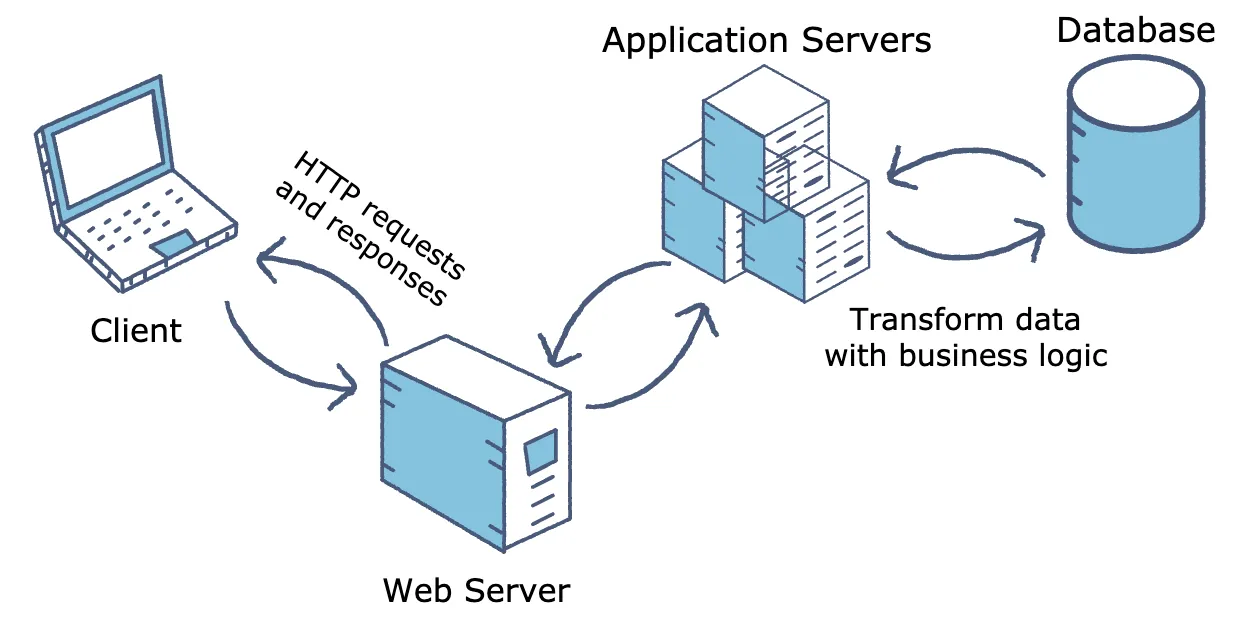
\includegraphics[width=0.7\textwidth]{slike/arh.png} %veličina u odnosu na širinu linije
	\end{center}

	Arhitektura sustava može se podijeliti na tri glavna podsustava:
	
	\begin{itemize}
		\item \textit {Web poslužitelj} je odgovoran za komunikaciju klijenta i web aplikacije. Klijent je web preglednik - prevoditelj koji stranicu pisanu u kodu interpretira u web stranicu razumljivu korisnicima.  Korisnik putem web preglednika šalje zahtjev web poslužitelju. Komunikacija se odvija protokolom za prijenos informacija na webu - HTTP (HyperText Transfer Protocol). Web poslužitelj prima zahtjeve od korisnika putem web preglednika i prosljeđuje ih web aplikaciji na daljnju obradu.
		
		\item \textit {Web aplikacija} predstavlja središte sustava i obrađuje zahtjeve koje prima od korisnika putem web poslužitelja. Ovisno o zahtjevu, pristupa bazi podataka kako bi dohvatila ili ažurirala podatke.
		
		\item \textit {Baza podataka} je podsustav za trajnu pohranu podataka koji se koriste u aplikaciji. Web aplikacija komunicira s bazom podataka kako bi dohvatila, ažurirala, brisala ili pohranila podatke prema korisničkim zahtjevima. Podaci se strukturirano pohranjuju i dohvaćaju putem upita. \newline
		
	\end{itemize}
	
		Arhitektura sustava temelji se na MVC (Model-View-Controller) konceptu. Ovaj pristup omogućuje jasnu podjelu odgovornosti unutar sustava, olakšava održavanje, testiranje i proširivost aplikacije. 
		
		\begin{center}
			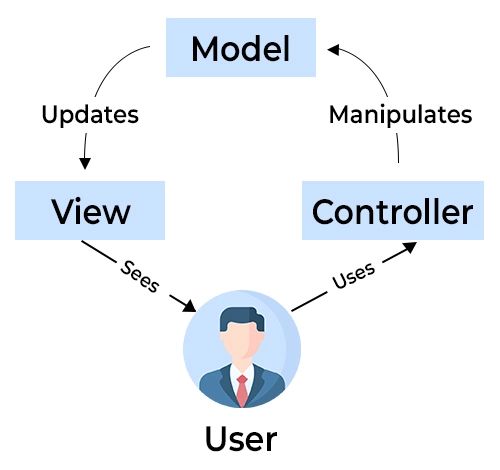
\includegraphics[width=0.4\textwidth]{slike/mvc.png} %veličina u odnosu na širinu linije
		\end{center}
		
		\begin{itemize}
			\item \textit{Model} predstavlja podatke i poslovnu logiku aplikacije. Model je odgovoran za dohvaćanje, pohranu i upravljanje podacima. Komunicira s Controllerom i obavještava ga o ažuriranim informacijama.
			
			\item \textit{View} predstavlja korisničko sučelje aplikacije. Sve što korisnik vidi je dio Viewa. On prikazuje podatke koje dobiva od Modela.
			
			\item \textit{Controller} je posrednik između Modela i Viewa. Prima korisničke zahtjeve iz Viewa, interpretira ih i odabire odgovarajuće akcije. Ovisno o korisničkom zahtjevu, Controller može ažurirati Model (kao što je spremanje podataka u bazu) i/ili ažurirati View (kao što je prikazivanje novih podataka na web stranici). Controller šalje informacije od Viewa prema Modelu, a zatim ažurirane podatke iz Modela šalje natrag Viewu za prikaz korisnicima.
		\end{itemize}
		
		 
		Aplikacija ima slojeve frontend i backend, te bazu podataka. Baza podataka zadužena za pohranu podataka naše web aplikacije je PostgreSQL. Iz nje backend sloj dohvaća podatke koristeći Spring Boot tehnologiju. Za frontend sloj koji korisniku prikazuje podatke koje dobiva iz backenda putem API-a koristimo Angular.
		

		

				
		\section{Baza podataka}
			
			\textbf{\textit{dio 1. revizije}}\\
			
		\textit{Potrebno je opisati koju vrstu i implementaciju baze podataka ste odabrali, glavne komponente od kojih se sastoji i slično.}
		
			\subsection{Opis tablica}
			

				\textit{Svaku tablicu je potrebno opisati po zadanom predlošku. Lijevo se nalazi točno ime varijable u bazi podataka, u sredini se nalazi tip podataka, a desno se nalazi opis varijable. Svjetlozelenom bojom označite primarni ključ. Svjetlo plavom označite strani ključ}
				
				
				\begin{longtblr}[
					label=none,
					entry=none
					]{
						width = \textwidth,
						colspec={|X[6,l]|X[6, l]|X[20, l]|}, 
						rowhead = 1,
					} %definicija širine tablice, širine stupaca, poravnanje i broja redaka naslova tablice
					\hline \SetCell[c=3]{c}{\textbf{korisnik - ime tablice}}	 \\ \hline[3pt]
					\SetCell{LightGreen}IDKorisnik & INT	&  	Lorem ipsum dolor sit amet, consectetur adipiscing elit, sed do eiusmod  	\\ \hline
					korisnickoIme	& VARCHAR &   	\\ \hline 
					email & VARCHAR &   \\ \hline 
					ime & VARCHAR	&  		\\ \hline 
					\SetCell{LightBlue} primjer	& VARCHAR &   	\\ \hline 
				\end{longtblr}
				
				
			
			\subsection{Dijagram baze podataka}
				\begin{figure}[H]
					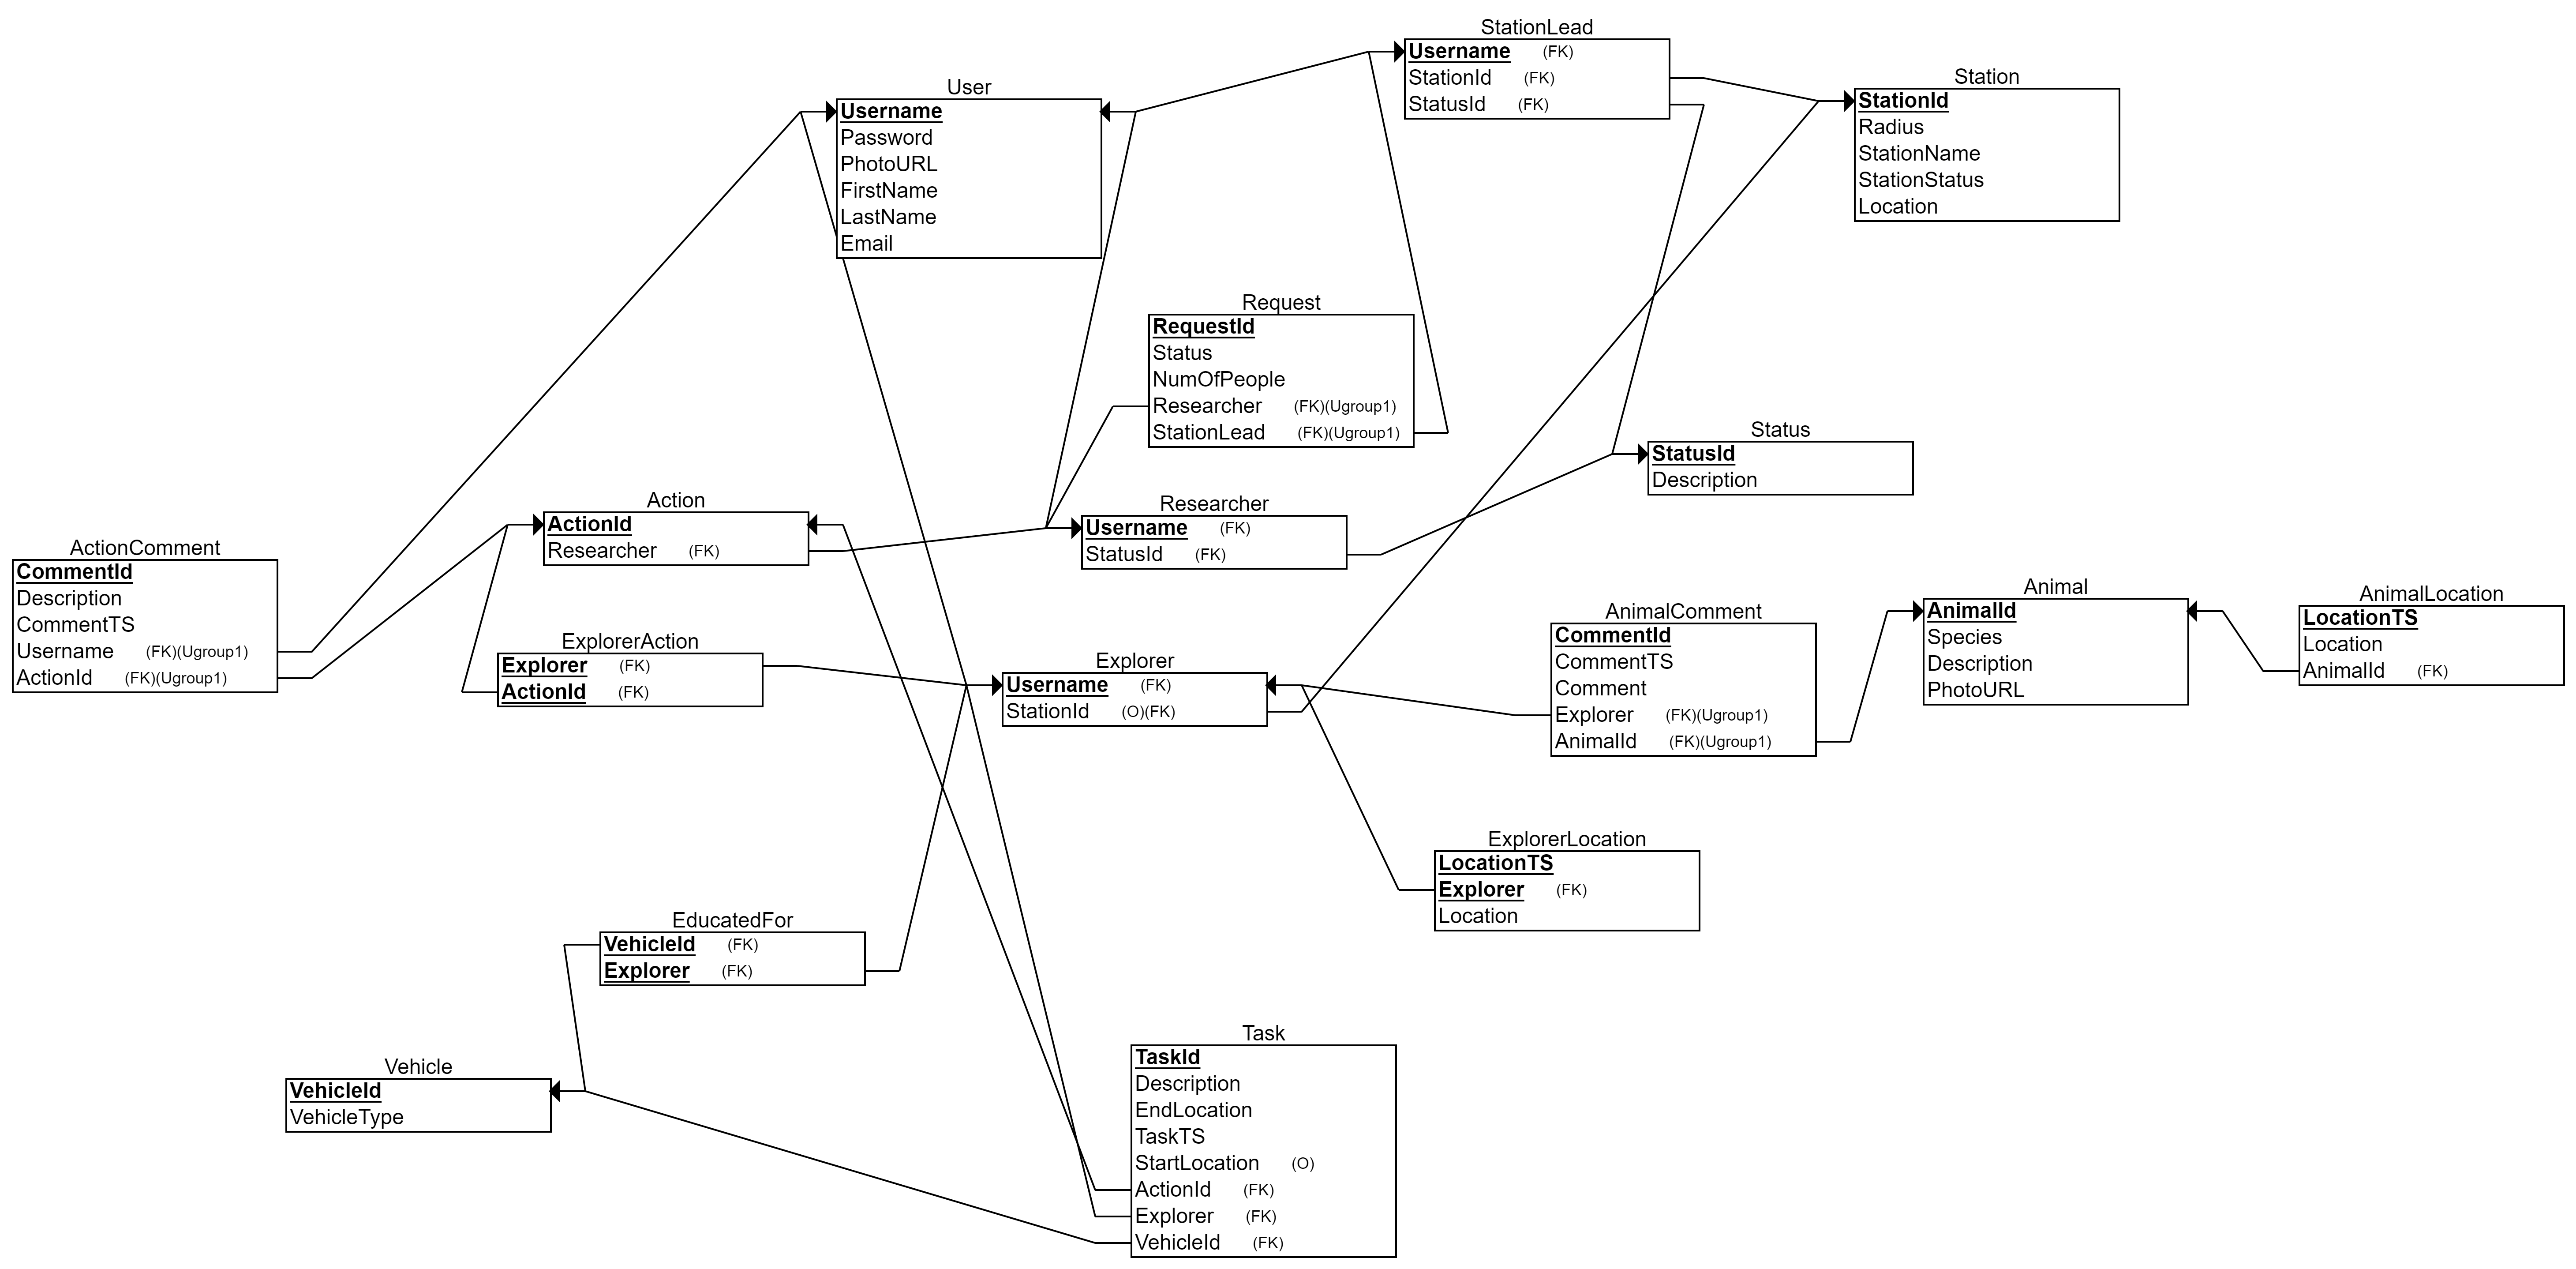
\includegraphics[width=\textwidth]{slike/dijagram_baze.PNG} %veličina u odnosu na širinu linije
					\caption{Dijagram baze podatatka}
					\label{fig:dijagram_baze} %label mora biti drugaciji za svaku sliku
				\end{figure}
			
			\eject
			
			
		\section{Dijagram razreda}
		
			\textit{Potrebno je priložiti dijagram razreda s pripadajućim opisom. Zbog preglednosti je moguće dijagram razlomiti na više njih, ali moraju biti grupirani prema sličnim razinama apstrakcije i srodnim funkcionalnostima.}\\
			
			\textbf{\textit{dio 1. revizije}}\\
			
			\textit{Prilikom prve predaje projekta, potrebno je priložiti potpuno razrađen dijagram razreda vezan uz \textbf{generičku funkcionalnost} sustava. Ostale funkcionalnosti trebaju biti idejno razrađene u dijagramu sa sljedećim komponentama: nazivi razreda, nazivi metoda i vrste pristupa metodama (npr. javni, zaštićeni), nazivi atributa razreda, veze i odnosi između razreda.}\\
			
			\textbf{\textit{dio 2. revizije}}\\			
			
			\textit{Prilikom druge predaje projekta dijagram razreda i opisi moraju odgovarati stvarnom stanju implementacije}
			
			
			
			\eject
		
		\section{Dijagram stanja}
			
			
			\textbf{\textit{dio 2. revizije}}\\
			
			\textit{Potrebno je priložiti dijagram stanja i opisati ga. Dovoljan je jedan dijagram stanja koji prikazuje \textbf{značajan dio funkcionalnosti} sustava. Na primjer, stanja korisničkog sučelja i tijek korištenja neke ključne funkcionalnosti jesu značajan dio sustava, a registracija i prijava nisu. }
			
			
			\eject 
		
		\section{Dijagram aktivnosti}
			
			\textbf{\textit{dio 2. revizije}}\\
			
			 \textit{Potrebno je priložiti dijagram aktivnosti s pripadajućim opisom. Dijagram aktivnosti treba prikazivati značajan dio sustava.}
			
			\eject
		\section{Dijagram komponenti}
		
			\textbf{\textit{dio 2. revizije}}\\
		
			 \textit{Potrebno je priložiti dijagram komponenti s pripadajućim opisom. Dijagram komponenti treba prikazivati strukturu cijele aplikacije.}